\chapter{Perturbation Theory}

The many body Schr\" odinger equation is rather difficult to solve. 
Even a two body problem is a rather complicated system to solve, that is why
we have to come up with approximated methods. Usually the Hamiltonian gets 
separated in an unperturbed part and a perturbed part, The perturbed part is
the one which considers the interactions between the particles. 

\be
H\Psi=(H_0 +V)\Psi=E\Psi.
\ee

$H_0$ is the unperturbed Hamiltonian, which is a one particle operator, 
which in most of the problems governing nuclear physics is a harmonic 
oscillator Hamiltonian. Then $H_0=E_{kin} + U_{H.O}$ and $V = V-U_{H.O}.$
Where $E_{kin}$ is the kinetic energy and $U_{H.O}$ is the harmonic oscillator potential. 
Obviously the difference $V-U_{H.O}$ should be small enough so that
 threating $V$ as a perturbation is valid. The exact result is independent of the one particle potential $U$, but 
in an approximated calculation it is possible that the results depend on the one particle potential that is included in
the calculations. The eigenfunctions, $\phi_i$ are taken as a basis for the expansion of the eigenfunction $\Psi$


\be
\ket{\Psi}=\sum_{i=1}a_i\ket{\phi_i}
\ee

It is common practice to divide the space in a model space and an excluded space, to simplify the calculations. By doing this we define 
two projection operators, that we will meet again later. These projection operators are denoted by a $P$ and a $Q.$ The $P$ operator projects
the complete wavefunction onto the model space 

\be
P\ket{\Psi}=\ket{\Psi_M}.
\ee


While $Q$ is the complimentary projector operator and projects the complete wavefunction to the excluded state $\ket{\Psi_Q}.$ 

\be
\begin{split}
P=\sum_{i=1}^d \ket{\phi_i}\bra{\phi_i}\\
Q=\sum_{i=d+1}^N \ket{\phi_i}\bra{\phi_i}\\
\end{split}
\ee
The projection operators satisfy the properties

\be
\begin{split}
P^2=P\\
Q^2=Q\\
PQ=QP=0\\
P+Q=1
\end{split}
\label{projectionopprop}
\ee

Since $e_k$ are the eigenvalues of the unperturbed Hamiltonian $H_0$, we obtain that 

\be
(E-e_j)a_j=\bra{\phi_j}V\ket{\Psi}.
\label{differense}
\ee

By using this relation we find that the entire wavefunction $\ket{\Psi}$ can be written as

\be
\ket{\Psi}= \sum_{i=1}^d a_i\ket{\phi_i} + \sum_{i=d+1}^N\frac{\ket{\phi_i}\bra{\phi_i}V\ket{\Psi}}{E-e_i}=\sum_{i=1}^da_i\ket{\phi_i} + \frac{QV}{E-H_0}\ket{\Psi}= P\ket{\Psi} + \frac{QV}{E-H_0}\ket{\Psi}
\ee

If we now define a wave operator which projects the model space onto the complete wavefunction $\Omega\ket{\Psi_M}=\ket{\Psi}$ we find it to be


\be
\Omega(E)=1 + \frac{Q}{E-H_0}V\Omega(E)
\ee

If we now use the wave operator in Eq \eqref{differense} we get 

\be
(E-e_j)a_j=\bra{\phi_j}V\Omega\ket{\Psi_M}=\sum_{k=1}^d\bra{\phi_j}V\Omega\ket{\phi_k}a_k
\ee

which is equivalent to 

\be
[H_0 + V\Omega(E) -E]\Psi_M=0.
\ee


If we define an effective interaction 

\be
\mathcal V(E)=V\Omega(E)
\ee

we get an integral equation, 

\be
\mathcal V(E)=V + V\frac{Q}{E-H_0}\mathcal V(\Omega),
\label{effektivvv}
\ee

for the effective interaction, which is dependent on the energy $E$. 
Eq. \eqref{effektivvv} can be solved by iteration, where we by using $V$ as
a first guess find that

\be
\begin{split}
&\mathcal V(E)=V + VQ\frac{1}{E-H_0}QV +VQ\frac{1}{E-H_0}QVQ\frac{1}{E-H_0}QV
+\\
& VQ\frac{1}{E-H_0}QVQ\frac{1}{E-H_0}QVQ\frac{1}{E-H_0}QV + \cdots
\end{split}
\ee

This can be solved analytically by observing that the sum resembles a 
geometric sum. 

\be
\begin{split}
\mathcal V=V + VQ\frac{1}{E-H_0-QVQ}QV\\
\equiv PVP + PVQ\frac{1}{E-QHQ}QVP
\end{split}
\ee


\section{Time dependent perturbation theory}


When doing time dependent perturbation theory we have to define the time 
evolution propagator $U(t,t')$, the time evolution operator evolve a state 
$\Psi(t')$ at time $t'$ to state $\Psi(t)$ at 
time $t$. 

\be
\Psi(t)=U(t,t')\Psi(t')
\ee

The wavefunctions satisfy the time dependent Schr\" odinger equation, 

\be
\begin{split}
&i\hbar \frac{\partial}{\partial t}\Psi(t)=H\Psi(t)\\
&i\hbar \frac{\partial}{\partial t}\Psi(t)=i\hbar \frac{\partial}{\partial t}U(t,t')\Psi(t'),
\end{split}
\ee

which yields that the time evolution operator satisfy Schro\" dinger equation. The solution is

\be
U(t,t')=e^{-iH(t-t')/\hbar}.
\ee


This form of the time evolution operator gives right away the properties one would expect of an
operator of this kind

\be
\begin{split}
&U(t,t)=1\\
&U(t',t)U(t,t')=1\\
&U(t,t')U(t,t')^\dagger=U(t,t')^\dagger U(t,t')=1\\
&\rightarrow U(t',t)=U(t,t')^\dagger=U(t,t')^{-1}\\
&U(t_1,t_2)U(t_2,t_3)=U(t_1,t_3)
\end{split}
\ee


By use of Thouless theorem \cite{thouless}, exact eigenstates can be constructed
through the action of the time-development operator.  In the present approach
the time $t$ will be rotated by a small angle $\epsilon$, our time is complex. 

The eigenstate can the be written as

\be
\frac{\ket{\psi_i}}{\braket{\phi}{\psi_i}}=\substack{lim\\ \epsilon \rightarrow 0}\, \substack{lim\\t'\rightarrow\\-\infty(1-i\epsilon)}
\frac{U(t,t')\ket{\phi}}{\bra{\phi}U(t,t')\ket{\phi}},
\label{eigenstatefortime}
\ee

where $\ket{\psi_i}$ is the lowest state of $H$ with $\braket{\phi}{\psi_i}\neq
0.$ This relationship is very useful in calculating the ground state energy
shift $\Delta E_0.$

If our unperturbed Hamiltonian gives the energy $E_0$ while acting on the
unperturbed state $\ket{\phi}$, and our total energy is $E$ the ground state
energy shift is given by

\be
\begin{split}
&\Delta E_0=E-E_0=\frac{\bra{\phi}V\ket{\psi}}{\braket{\phi}{\psi}}\\
&=\substack{lim\\ \epsilon \rightarrow 0^+}\substack{lim \\t'\rightarrow \\
 -\infty(1-i\epsilon)}\frac{\bra{\phi}VU(0,t')\ket{\phi}}{\bra{\phi}U(0,t')\ket{\phi}}
\label{energyshift1}
\end{split}
\ee

To evaluate this as a perturbation, we have to expand the time evolution
operator $U(t,t')$. This is most conveniently if it is done in the interaction
picture. Which will be explained slightly here, \cite{shankar94} and
\cite{sakurai} give a more thoroughly explanation of the interaction picture. 
The interaction picture can be understood as an intermediate between the Schr\" odinger picture and the Heisenberg picture. In the Schr\" odinger picture the 
operators are time independent while the state evolves with time. It is all
contrary in the Heisenberg picture where the operators now are time dependent
and the state is time independent.
In the interaction picture both the state vectors and the operators are time
dependent, however their time dependencies are somewhat different.

A state vector in the interaction picture is defined as

\be
\ket{\psi_I(t)}=e^{iH_{0,S}t/\hbar}\ket{\psi_s(t)}
\ee


where the letter $S$ stands for the schr\" odinger picture. The operators in the interaction picture is defined as

\be
A_{I}(t) = e^{i H_{0,S} t / \hbar} A_{S}(t) e^{-i H_{0,S} t / \hbar}. 
\ee

$H_0$ is still the unperturbed Hamiltonian. The time evolution of the operators is given by 

\be
i\hbar\frac{d}{dt}A_I(t)=\left[A_I(t),H_0\right].\; 
\ee



By using the definition of one particle and two particle operators from chapter
\ref{chapsecondq}, our Hamiltonian can be written as in Eq.
 \eqref{hamiltoniansec}


\be
H=\sum_{k} \epsilon_{k}a^\dagger_ka_k + \frac{1}{2}\sum_{ijkl}V_{ijkl}a^\dagger_i
a^\dagger_ja_la_k.
\ee

To find the time evolution of  the Hamiltonian it suffices to find the time
evolution of the creation and annihilation operators $a^\dagger$ and $a.$
Using the commutator we find that

\be
\left[a^\dagger_k,H_0\right]=-\epsilon a^\dagger_k(t)
\ee

thus we obtain the time dependence of the creation and destruction operators

\be
\begin{split}
& a^\dagger(t)_k=a^\dagger_ke^{i\epsilon_kt/\hbar}\\
& a(t)_k=a_ke^{-i\epsilon_kt/\hbar}
\end{split}
\ee

I will now transform the schr\" odinger equation to the interaction picture

\be
\begin{split}
&\psi_I(t)=e^{iH_0t/\hbar}\psi(t)\\
&=e^{iH_0t/\hbar}U(t,t')e^{-iH_0t'/\hbar}e^{iH_0t'/\hbar}\psi(t')\\
&=U_I(t,t')\psi_I(t')
\end{split}
\label{itertimeop}
\ee

By differentiating Eq. \eqref{itertimeop} with respect to time $t$ we find

\be
\frac{\partial}{\partial t}U(t,t')=VU(t,t')
\ee

When we have found how the time evolution operator we may also find the 
perturbartive expansion of the time evolution operator. The solution to the differential equation is 

\be
U(t,t')=1 +\left(\frac{-i}{\hbar}\right) \int_{t'}^tdt_1V(t_1)U(t_1,t')
\label{ekspavtidev}
\ee


The number 1 in Eq. \eqref{ekspavtidev} is for satisfying $U(t',t')=1.$
Eq. \eqref{ekspavtidev} can be solved by iteration

\be
U(t,t')=1+\sum_{n=1}^\infty\left(\frac{-i}{\hbar}\right)^n\int_{t'}^tdt_1
\int_{t'}^{t_1}dt_2\cdots \int_{t'}^{t_{n-1}}dt_nV(t_1)V(t_2)\cdots V(t_n)
\ee

Now the above form of the time evolution operator can be inserted into Eq. 
\eqref{eigenstatefortime}, which gives us the perturbative expansion for
calculating the interactions.


\section{Feynman-Goldstone diagrams}

To evaluate Eq. \eqref{eigenstatefortime} we had to define a new operator, called the time ordering operator. The effect of operating this operator on a 
product of operators is to order the operators so the operators with a larger
time argument are placed to the left to those of smaller time arguments. Since we in nuclear physics are dealing with fermions which obey the Pauli exclusion
principle there will be a sign dependency on the number of permutations needed 
in making the arrangement. As an example 

\be
\begin{split}
T\left[A_1(t_1)A_2(t_2)\cdots A_n(t_n) \right]\\
=(-1)^pA_\alpha(t_\alpha)A_\beta(t_\beta) \cdots A_\gamma(t_\gamma)
\end{split}
\ee

If we use time ordering together with the particle hole formalism from section \ref{particlehole}, we will find a new definition of the contraction.
A contraction of two operators will now be defined as

\be
\wick{1}{<1A>1B}=T[AB]-N[AB], 
\ee

Where $N[AB]$ is the normal ordering operator. 
As an example I will derive a contraction 
of two hole operators and a contraction of two particle operators. 
I will first start with a contraction of two hole operators where both 
particles have momenta below $k_F,$ and with $t < t'.$


\be
\begin{split}
&\wick{1}{<1a_h(t)>1a_{h'}^\dagger (t')}=T\left[a_h(t)a_{h'}^\dagger (t')\right]
-N\left[a_h(t)a_{h'}^\dagger (t')\right]\\
&=-a_{h'}^\dagger (t')a_h(t)-a_h(t)a_{h'}^\dagger(t')\\
&=-\left(a^\dagger_{h'}(t')a_h(t)+a_h(t)a_{h'}^\dagger(t')\right)e^{-\frac{i}{\hbar}(\epsilon_ht-\epsilon_{h'}t')}\\
& = -\delta_{h,h'}e^{-\frac{i}{\hbar}(\epsilon_ht-\epsilon_{h'}t')}.
\end{split}
\label{kontrakt1}
\ee

Similarly for particles with momenta above $k_F$ and $t<t'$

\be
\wick{1}{<*a_p(t)>*a_{p'}(t')}=\delta_{p,p'}e^{-\frac{i}{\hbar}\epsilon_p(t-t')}
\label{kontrakt2}
\ee

We have 

\be
\wick{1}{<*a_\alpha(t)>*a_\beta^\dagger(t')}=-\wick{1}{<*a_\beta^\dagger(t')>*a_\alpha(t)}
\ee

\begin{figure}[htp]
\centering
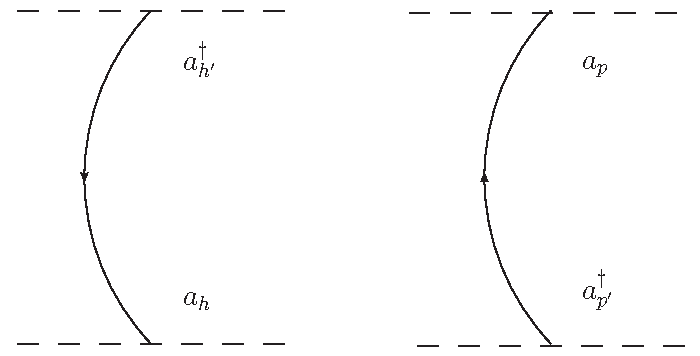
\includegraphics[scale=0.5]{hullpartlinje}
\caption{Diagrammatic representation of the contractions in Eqs. 
\eqref{kontrakt1} and \eqref{kontrakt2} The time is going upward.}
\label{hullpartlinje}
\end{figure}

In Fig (\ref{hullpartlinje}) the two contractions in Eqs \eqref{kontrakt1} 
and \eqref{kontrakt2} are represented diagrammatically, the annihilation 
operator $a_\alpha$ destroys the particle line $a^\dagger_\beta$ creates. The
time is upward.

With the above definitions of time ordering and contractions we are ready to go back to the time evolution operator, it is already in a time ordered 
form.

\be
U(t,t')=\sum_{n=0}^\infty\left(\frac{-i}{\hbar}\right)^n\int_{t'}^tdt_1
\int_{t'}^{t_1}dt_2\cdots \int_{t'}^{t_{n-1}}dt_nT\left[V(t_1)V(t_2)\cdots V(t_n)\right]
\label{tidevolusjon1}
\ee

From  Eq. \eqref{tidevolusjon1} we see that the integral with respect to the time $t_1,t_2 \cdots t_n$ and that there are $n!$ ways to order them, we can again rewrite the time evolution operator in the form



\be
U(t,t')=\sum_{n=0}^\infty\frac{1}{n!}\left(\frac{-i}{\hbar}\right)^n\int_{t'}^tdt_1
\int_{t'}^{t}dt_2\cdots \int_{t'}^{t}dt_nT\left[V(t_1)V(t_2)\cdots V(t_n)\right]
\label{tidevolusjon2}
\ee


If we recall that it is the energy shift we want to calculate, we can rewrite Eq. \eqref{energyshift1}



\be
\begin{split}
&\Delta E_0=\substack{lim\\ \epsilon \rightarrow 0^+}\substack{lim \\t'\rightarrow \\
 -\infty(1-i\epsilon)}\frac{\bra{\phi}VU(0,t')\ket{\phi}}{\bra{\phi}U(0,t')\ket{\phi}}\\
&=\sum_{n=0}^\infty\frac{1}{n!}\left(\frac{-i}{\hbar}\right)^n\int_{t'}^tdt_1
\int_{t'}^{t}dt_2\cdots \int_{t'}^{t}dt_n\bra{\phi}T\left[V(t)V(t_1)V(t_2)\cdots V(t_n)\right]\ket{\phi}\\
&\times \frac{1}{\sum_{n=0}^\infty\frac{1}{n!}\left(\frac{-i}{\hbar}\right)^n\int_{t'}^tdt_1
\int_{t'}^{t}dt_2\cdots \int_{t'}^{t}dt_n\bra{\phi}T\left[V(t_1)V(t_2)\cdots V(t_n)\right]\ket{\phi}}.
\end{split}
\label{energyshift2}
\ee

Where $V(t)$ in the numerator in  Eq. \eqref{energyshift2} is put into to 
the time ordering operator. 
To evaluate the integrals in the numerator and the
denominator we have to use wicks theorem, wicks theorem with time ordering
will be slightly modified from the first version in section \ref{wicksteorem}. Wicks theorem states now that 

\be
\begin{split}
&T\left[A(t_1)B(t_2)C(t_3) \cdots Z(t_n)\right]=N\left[A(t_1)B(t_2)C(T_3) \cdots Z(t_n)\right]\\
&+ \sum_{1\, contraction}N\left[A(t_1)B(t_2)C(T_3) \cdots Z(t_n)\right]+\sum_{2\, contractions}N\left[A(t_1)B(t_2)C(T_3) \cdots Z(t_n)\right]\\
&+ \cdots + \sum_{\substack{contractions\, with\\ all \, operators}}N\left[A(t_1)B(t_2)C(T_3) \cdots Z(t_n)\right]\\
\end{split}
\label{wicktheofortime}
\ee

Since our unperturbed state is the groundstate, which is our reference vacuum state, only the last term in Eq. \eqref{wicktheofortime} survive. We are 
left with the term where all operators are participating in the contractions.

Let us now evaluate the first order contribution to the energy shift in Eq. \eqref{energyshift2}. The only contributing term is $V(t)$ which in 
a second quantized form is $V_{\alpha\beta\gamma\delta}a^\dagger_\alpha(t) a^\dagger_\beta(t) a_\delta(t) a_\gamma(t).$
From wicks theorem we will then have two terms contributing to the energy shift.

\be
\begin{split}
\wick{21}{<*a^\dagger_\alpha(t) <2a^\dagger_\beta(t) >2 a_\delta(t) >*a_\gamma(t)} +
\wick{21}{<*a^\dagger_\alpha(t) <2a^\dagger_\beta(t) >* a_\delta(t) >2a_\gamma(t)} 
\end{split}
\label{forsteordenbidrag}
\ee


The terms in Eq. \eqref{forsteordenbidrag} can be depicted diagrammatically 
as seen in Fig (\ref{forsteordendiagram}).

\begin{figure}[htp]
\centering
%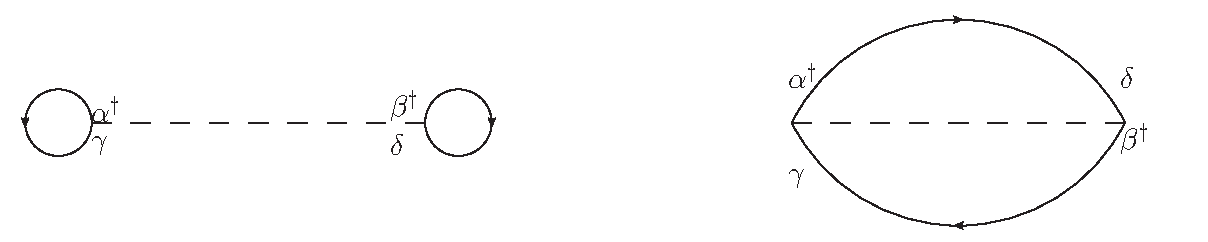
\includegraphics[height=0.8\textheighti]{forsteordendiagram}
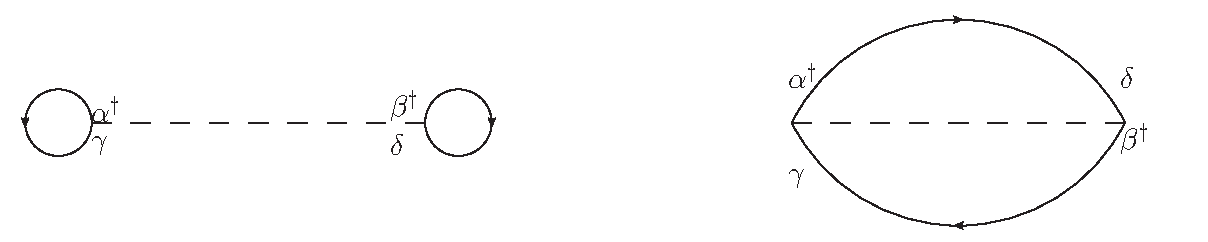
\includegraphics[scale=0.5]{forsteordendiagram}  %[width=1.0\textwidth]{forsteordendiagram}
\caption{Diagrammatic representation of the first order diagram, the diagram to the left depicts the first term in Eq. \eqref{forsteordenbidrag}, the 
diagram to the right depicts the second term in Eq. \eqref{forsteordenbidrag}.}
\label{forsteordendiagram}
\end{figure}

$\alpha, \, \beta, \, \gamma$ and $\delta$ must all be holes, since they are all equal time operators and hence the only contractions which contribute.
The energy shift can now be written as 

\be
\Delta E_0=	 \frac{1}{2}\sum_{\alpha\beta < k_f} \frac{1}{2}(V_{\alpha\beta\alpha\beta}-V_{\alpha\beta\beta\alpha})
\ee

The minus sign comes in, by the "rule" that for every contraction that cross
another contributes with a factor $(-1).$

With the clever invention of the diagrams that depicts the contractions, we are
able to describe every term in the expansion of the time evolution operator as
diagrams. These diagrams are usually called Feynman diagrams or
Feynman-Goldstone diagrams, to honor the inventor.  When presenting all the
terms as diagrams we need some rules to keep track of them. The idea is that we
find a term in the expansion by studying the corresponding diagram. A nice derivation of the diagram
rules can be found in \cite{kuo1981}.  The rules are described in appendix
\ref{diagramregler}. 




